\section{Introduction}
\label{s:intro}
Due to the broadcast nature of wireless channels, considerable attention has been given to the security and privacy aspects of wireless communications. While the content of messages (i.e., the information transmitted over the channel) can be protected against unauthorized access using cryptography or physical-layer security techniques \cite{zhou2013physical}, there are occasions when hiding the very existence of the communication channel is as vital as securing the communicated messages themselves. Examples of such situations include military operations, cyber espionage, social unrest, or privacy concerns of communication parties. All of the aforementioned use cases have motivated the study of hidden communication channels, which are referred to as ``covert communication'' \cite{lampson1973note, bloch2016covert} in the literature.

The preliminary attempt to obtain covertness started with the study of spread spectrum almost a century ago, with the main purpose of hiding military communications \cite{scholtz1982origins}. The idea was to transmit the signal over a wide frequency band, which would make it harder to locate and identify the original signal amidst the background noise. Many works continued to further examine different aspects of this idea \cite{reynders2016chirp, yan2019low}. However, the fundamental performance limits of such work were unknown until recently when Bash et al. \cite{bash2012square, bash2013limits} established a square root limit on the number of covert bits that can be reliably sent over an additive white Gaussian noise (AWGN) channel. Following this work, there has been a surge of interest in examining covert channels \cite{sobers2017covert,soltani2018covert,sheikholeslami2018multi,cao2018wireless}.

Numerous works have studied the theoretical limits of covert communication over wireless systems in different scenarios \cite{bash2012square, soltani2018covert, sheikholeslami2018multi, li2021fundamental}, but only a few works have focused on the practical implementation of covert communication \cite{dutta2012secret, cao2018wireless, liao2020generative, mohammed2021adversarial}. Many of these works involve an external factor that covert users rely on to build their covert communication, such as hardware impairments \cite{mohammed2021adversarial}, the presence of a cooperative jammer \cite{sobers2017covert}, or the cooperation of a relay node \cite{liao2020generative, kim2022covert}. Additionally, the majority of works make some favorable assumptions for covert users, such as the existence of a shared secret key between covert users unknown to detector \cite{soltani2018covert}, the accessibility of covert users to cover signals and modulation type \cite{grzesiak2021wireless}, uncertainty in the knowledge of noise power at the detector's receiver \cite{he2017covert}, neglecting the impact of the covert system on normal communication \cite{mohammed2021adversarial}, and limiting the channel model to AWGN \cite{mohammed2021adversarial}. Imposing such restricted assumptions and dependencies eliminates the generality of these covert models and makes it difficult for them to adapt to different system deployments with distinct conditions. Last but certainly not least, recent studies show that covert communication that causes noticeable divergence in the statistical properties of signals can be easily detected using analytical and steganalysis methods \cite{bahramali2021robust,huang2020exploiting}.

There is a large body of work that focuses on different schemes of covert communication applied to traditional wireless systems. However, wireless systems research has greatly expanded in recent years to consider the potential impact of machine learning (ML) approaches for a variety of problems \cite{wang2017deep}. In fact, various network optimization problems, which were traditionally handled using statistical models, now leverage machine learning techniques \cite{zhu2020toward}. Deep neural networks (DNNs) in particular, the major force in machine learning, have helped address several wireless problems, such as signal classification \cite{o2016radio, o2017introduction, wu2020deep, makkuva2021ko}, channel estimation \cite{soltani2019deep}, transmitter identification \cite{roy2019rfal, hanna2019deep}, jamming, and anti-jamming \cite{arjoune2020novel, bahramali2021robust}. In a recent study, an end-to-end communication model based on deep learning emerged as a replacement for conventional modular-based designs \cite{o2017introduction}. In this new paradigm, the transmitter and receiver are designed based on DNNs that are jointly trained as the encoder and decoder of an autoencoder network \cite{o2017introduction}. The autoencoder network can be trained to learn the characteristics of the signal, such as its statistical properties, to develop modulation and coding techniques through a self-learning process. This eliminates the need for hand-crafted methods, giving the system the ability to determine the most effective way to modulate and encode data. Compared to traditional communication systems, this approach offers greater flexibility and robustness, as the autoencoder can adapt to varying channel conditions and noise levels without manual tuning \cite{zou2021channel}. Despite these benefits, Autoencoder wireless systems, similar to many other deep learning models, are highly susceptible to adversarial attacks \cite{chakraborty2018adversarial}, such as jamming \cite{bahramali2021robust}, spoofing attacks \cite{shi2020generative}, signal misclassification \cite{sadeghi2019physical}. This motivates us to study the vulnerabilities that ML-based wireless communication systems might have against covert communications.

\begin{figure}[tp!]
	\center
	\begin{subfigure}{0.45\textwidth}
		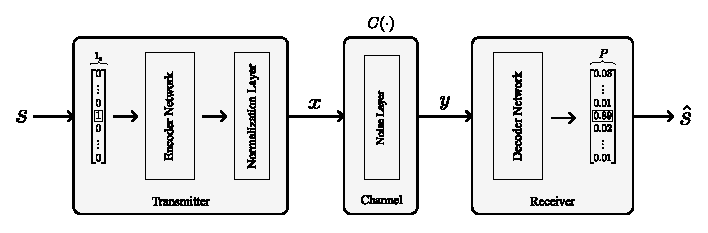
\includegraphics[width=\linewidth]{figs/original_autoencoder_architecture.eps}
	\end{subfigure}
	\\
	\caption{An end-to-end autoencoder-based communication system. The system receives a message \(s\) as input and generates a probability distribution over all possible messages. The most probable message is then selected as the output \(\hat{s}\) \cite{o2017introduction}.}	
	\label{fig:original_autoencoder_architecture}
\end{figure}

In this work, we introduce a novel deep learning-based covert communication scheme that is free of many aforementioned assumptions. It merely relies on the existing channel's noise effect and is independent of any external factor. Our scheme also requires no knowledge of the cover signals or the modulation type. Remarkably, in communication scenarios with a single normal user, our scheme does not even need knowledge about the type of the communication channel. Finally, by training our covert models in an adversarial setting against the observer and minimizing the impact of the covert communication on ongoing normal communication, we ensure that our added covert signals do not cause any conspicuous deviation in the statistical properties of the normal signals. This prevents our covert signals from being easily detected using analytical tools. It is also worthwhile to mention that even though we are proposing our method for autoencoder-based wireless communication systems, there is no limitation on integrating our model into existing conventional wireless communication systems.

The contributions of this work can be expressed as follows:
\begin{enumerate}
	\item \textbf{Cover-Agnostic}: We propose a novel covert communication approach using GANs that utilizes an input-agnostic generator and discriminator network to represent the covert sender and detector, respectively. These components are trained adversarially in a similar fashion to GANs, allowing our scheme to be independent of cover signals, waveforms, and modulation types used in wireless systems.
	\item \textbf{Channel Independent}: Our covert communication scheme is trained on three different channel models, including AWGN, Rayleigh Fading, and Rician Fading. We have conducted various experiments to demonstrate that our model can be trained to adapt to different channel conditions and is robust against various noise levels. Additionally, our scheme can be trained to operate on the channel without any prior knowledge of the channel model or noise characteristics.
	\item \textbf{Single-/Multi-User Adaptability}: We demonstrate that our scheme can be integrated into communication systems with both single and multi normal users, and it is robust to channel interference. We also show that there is a degree-of-freedom effect in our scheme, where increasing the number of users affects the performance of the covert and normal communication systems in the fading channels.
	\item \textbf{Controlled Trade-off between Covertness and Performance}: Our training procedure enables us to attain any desired trade-off between the level of covertness and the system's performance (i.e., communication rate) through the control of a set of independent control "knobs", independent of the channel characteristics or user messages.
	\item \textbf{Undetectability}: We have developed a training procedure based on the generative adversarial framework that involves Willie as a discriminator network and normal receiver's loss as a regularizer during training. This reduces the detection probability of covert signals while keeping the normal communication of system users unaffected.
\end{enumerate}
